\documentclass{article}

% Language setting
% Replace `english' with e.g. `spanish' to change the document language
\usepackage[english]{babel}

% Set page size and margins
% Replace `letterpaper' with `a4paper' for UK/EU standard size
\usepackage[letterpaper,top=2cm,bottom=2cm,left=3cm,right=3cm,marginparwidth=1.75cm]{geometry}

% Useful packages
\usepackage{amsmath}
\usepackage{graphicx}
\usepackage{amssymb}
\usepackage{array}
\usepackage[colorlinks=true, allcolors=blue]{hyperref}

\title{Finch: A Datastructure-Driven Array Programming Language}
\author{Willow Ahrens, Teo Collin, Radha Patel, Kyle Deeds, Changwan Hong, Saman Amarasinghe}

\begin{document}
\maketitle

\begin{abstract}
From FORTRAN to Numpy, arrays have revolutionized how we express computation.
Arrays are the highest-performing datastructure with a long history of investment and innovation, from hardware support to compiler technology. 
However, arrays can only handle dense rectilinear integer grids. Real world arrays often contain underlying structure, such as sparsity, runs of repeated values, or symmetry. We describe a compiler, Finch, which adapts existing programs and interfaces to the structure and sparsity of the inputs. Finch enables programmers to capture complex, real-world data scenarios with the same productivity they expect from dense arrays. Our approach enables new loop optimizations across multiple domains, unifying techniques such as sparse tensors, databases, and lossless compression. 
\end{abstract}

\section{Introduction}

%- Fortran supported lots of control structures, no data structures, just dense arrays.
%
%- We tried to emulate complex data using only dense arrays but with complicated control structures.
%
%- Recently, people tried to build frameworks to support structured data, but gave up a lot of program side
%
%- We’re bringing these together, both need to work together.
\subsection{Contributions}

\begin{enumerate}
\item A rich structured array programming language with for-loops
and complex control flow constructs at the same level of productivity
of dense arrays. To our knowledge, the Finch programming language is the first
to support if-conditions, early breaks, and multiple left hand sides over
structured data, as well as complex accesses such as affine indexing or scatter/gather.
\item More complex array structures than ever before. A complete level-by-level
structure-description language for expressing the structure of data
hierarchically. The first such set of formats to efficiently capture banded,
triangular, run-length-encoded, or sparse datasets, and any combination thereof.
\item The Finch compiler specializes programs to data structures in a
predictable, deterministic approach, making it easier to search the complex
space of programs and datastructures to find an appropriate fit for a given
application. The tensor interface makes it easy to extend Finch to new level
formats. A unique tensor lifecycle model enables polymorphism by analyzing the
appropriate stages to insert simple, overloadable, interface functions such as
initialization or finalization. 

\item We evaluate the productivity of our language in several case studies,
showing that Finch can be used to accelerate a wide range of applications, 
from classic operations such as spmv and spgemm, to more complex applications such as image processing and graph analytics.
We also demonstrate how Finch can fuse high-level operations to achieve a significant speedup over non-fused kernels. Additionally, as a case study, a high-level array programming language and fusion interface for
operations such as map, broadcast, or reduce that can be compiled to efficient
code using the previous loop-level abstractions.
%\item A complete set of level formats for expressing data patterns hierarchically in FiberTree-style decompositions. The first such set of formats to efficiently capture banded, triangular, run-length-encoded, or sparse-run-length-encoded datasets. The formats capture many use cases, from random updates to sequential construction.
%\item The Finch array language, mirroring simple for-loops with imperative code blocks and if-conditions. The first array programming language for the above data formats to support multiple outputs, affine indexing, and imperfectly-nested loops.
%\item Tensor lifecycles, a simple constraint on tensor reads and writes that elegantly restricts Finch programs to avoid complex data dependencies, and enables tensor polymorphism by providing implementers with well-defined functions to overload.
%\item Wrapper Tensors which modify existing datastructures and recombine them to support new patterns, such as affine indexing, padding, transposition, and slicing.
%\item Wrapper Levels which modify existing datastructures and enabling complex features such as atomic updates or contiguous versus separate allocation.
%\item We define the first mappings from the existing pydata/sparse array api high-level operations to low level finch notation
%\item <Performance Contributions>
\end{enumerate}

\begin{table}[h!]
\centering
\begin{tabular}{l|ccccc}
\textbf{Feature / Tool} & \textbf{Halide} & \textbf{Taco} & \textbf{Cora} & \textbf{Taichi} & \textbf{Finch} \\
\hline
Einsums and Contractions & \checkmark & \checkmark & \checkmark & \checkmark & \checkmark \\
Parallelism             & \checkmark & \checkmark & \checkmark & \checkmark & \checkmark \\
Multiple LHS            & \checkmark &            & \checkmark & \checkmark & \checkmark \\
Affine Indices          & \checkmark &            &            & \checkmark & \checkmark \\
Recurrence              & \checkmark &            &            &            &            \\
If-Conditions and Masks & \checkmark & \checkmark &            & \checkmark & \checkmark \\
Scatter Gather          & \checkmark &            &            & \checkmark & \checkmark \\
Early Break             &            & \checkmark &            &   \checkmark         & \checkmark \\
\end{tabular}
\caption{Feature support across various tools.}
\label{tab:features}
\end{table}

\begin{table}[h!]
\centering
\begin{tabular}{l|ccccc}
\textbf{Feature / Tool} & \textbf{Halide} & \textbf{Taco} & \textbf{Cora} & \textbf{Taichi} & \textbf{Finch} \\
\hline
Dense                    & \checkmark & \checkmark & \checkmark & \checkmark & \checkmark \\
Padded                   & \checkmark &            &            &            & \checkmark \\
One Sparse               &            & \checkmark &            & \checkmark & \checkmark \\
Sparse                   &            & \checkmark &            &            & \checkmark \\
Run-length               &            &            &            &            & \checkmark \\
Symmetric                &            &            &            &            & \checkmark \\
Regular Sparse Blocks    &            & \checkmark &            &            & \checkmark \\
Irregular Sparse Blocks  &            &            &            &            & \checkmark \\
Ragged                   &            &            & \checkmark &            & \checkmark \\
\end{tabular}
\caption{Support for various data structures across tools.}
\label{tab:data_structures}
\end{table}

\section{Background}
\subsection{Looplets}
\subsection{FiberTrees}

\subsection{Concordant Iteration}

\subsection{Protocols}

\section{The Finch Language}

\subsection{Syntax and Semantics}

\section{The Tensor Interface}

\subsection{Tensor Lifecycle, Declare, Freeze, Thaw, Unfurl}

\subsection{Level Abstraction}
    
\begin{enumerate}
\item fibers
\item assembly
\item reassembly
\end{enumerate}

\subsection{Core Level Langage Primitives}
\begin{enumerate}
\item SparseList
\item SparseDict
\item ...
\end{enumerate}

\subsection{Wrapper Tensors}

\subsection{Scalars}

\subsubsection{Sparse Scalars}
\subsubsection{Early Break Scalars}


\section{The Finch Compiler}

\subsection{Dimensionalization}

\subsection{Concordization}

\subsection{Bounds Analysis}

\subsection{Performance Warnings}

\subsection{Wrapperization}

\subsection{Simplification and Algebraic Transformations}


\section{Evaluation}

\subsection{Data-Driven Performance Engineering}
\subsubsection{Sparse-Sparse Matrix Multiply}
Examples that demonstrate performance engineering in a datastructure-driven model

\subsubsection{SpMV}

%Here's a figure with spmv_performance_sorted_(faster_than_taco).png and spmv_performance_sorted_(slower_than_taco).png

\begin{figure}
    \begin{minipage}[t]{0.5\textwidth}
        \vspace{0pt} % Add this to ensure top alignment within minipage
        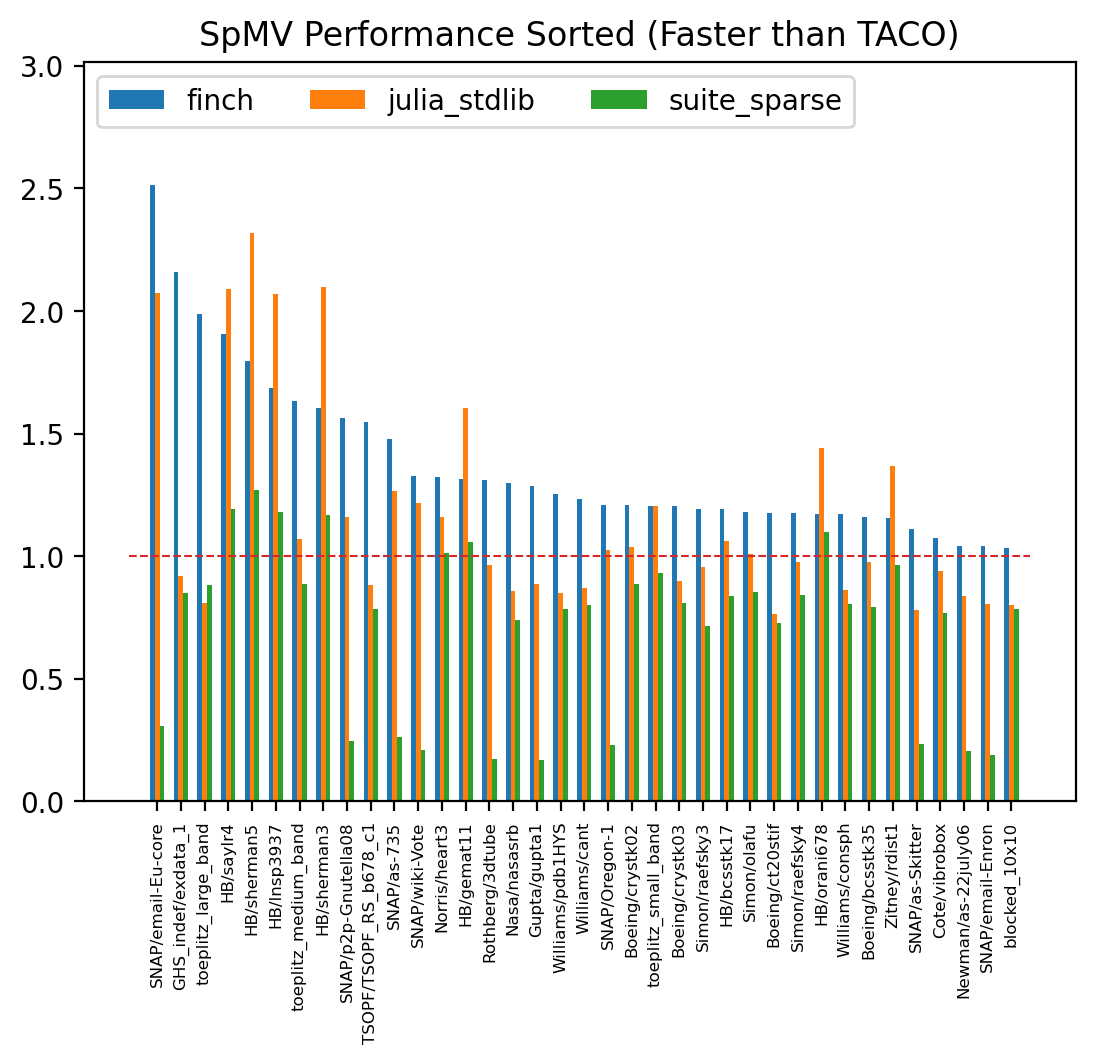
\includegraphics[width=\linewidth]{spmv_performance_sorted_(faster_than_taco).png}
    \end{minipage}%
    \begin{minipage}[t]{0.5\textwidth}
        \vspace{0pt} % Add this to ensure top alignment within minipage
        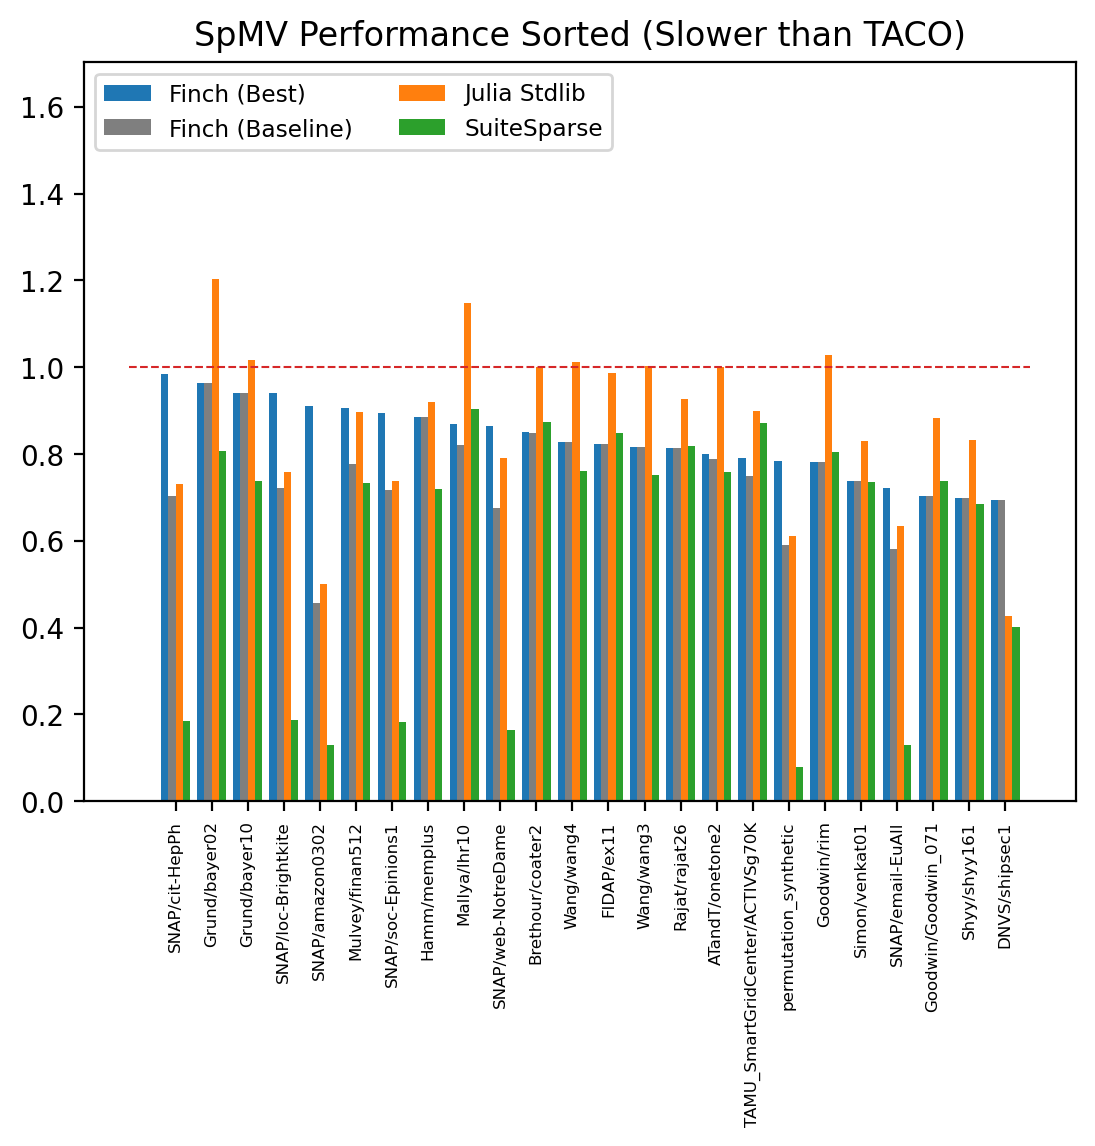
\includegraphics[width=\linewidth]{spmv_performance_sorted_(slower_than_taco).png}
    \end{minipage}
    \caption{Performance of SpMV across various tools.}
\end{figure}

\begin{figure}
    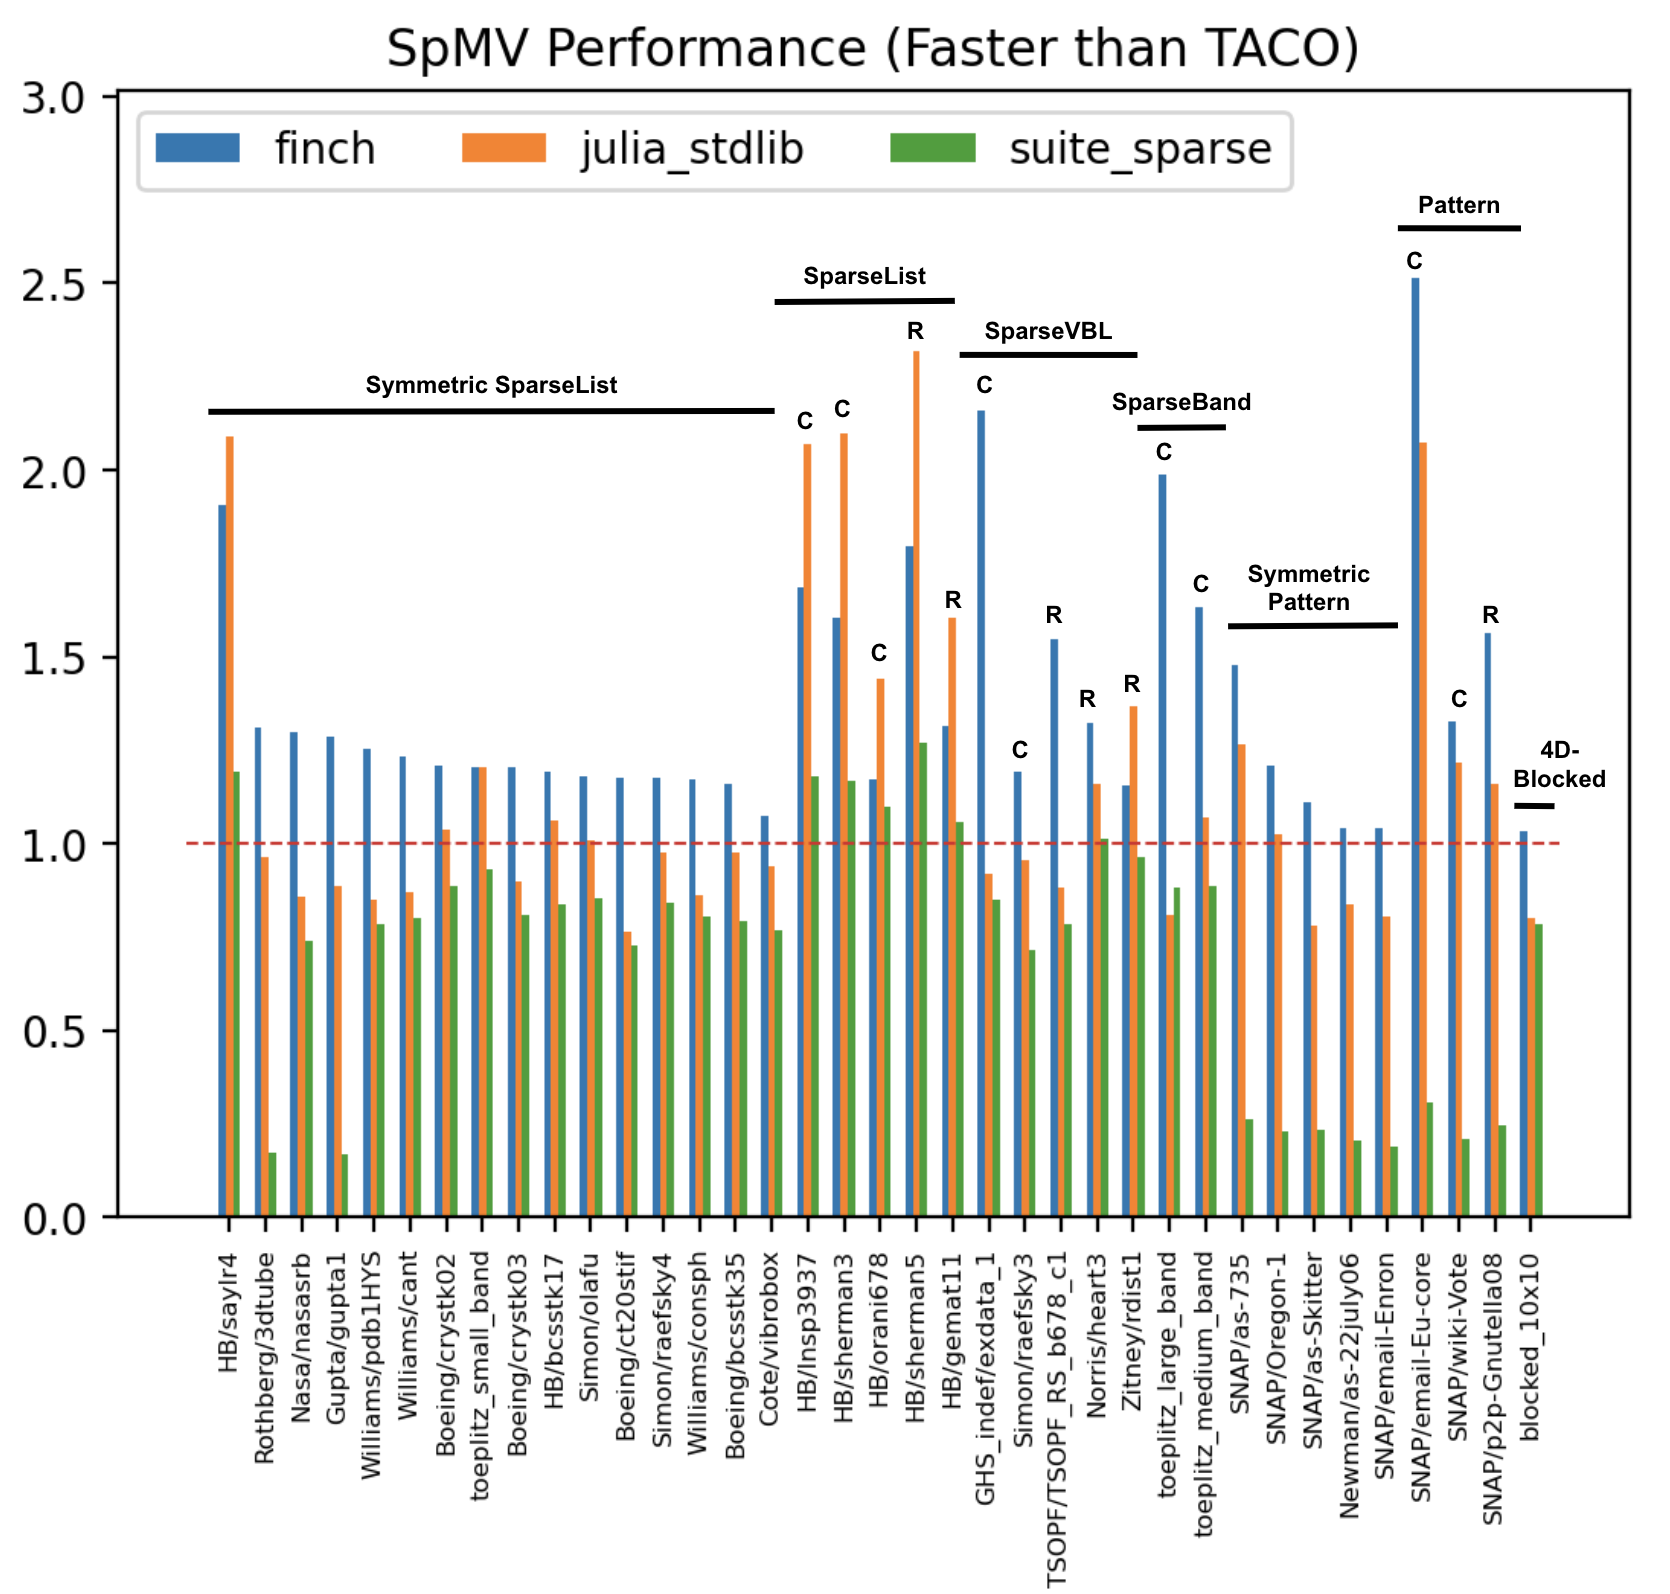
\includegraphics[width=\linewidth]{spmv_performance_grouped.png}
    \caption{Performance of SpMV by Finch format.}
\end{figure}


\subsection{Programming over flexible data}

\subsubsection{Image Morphology}

\begin{figure}
	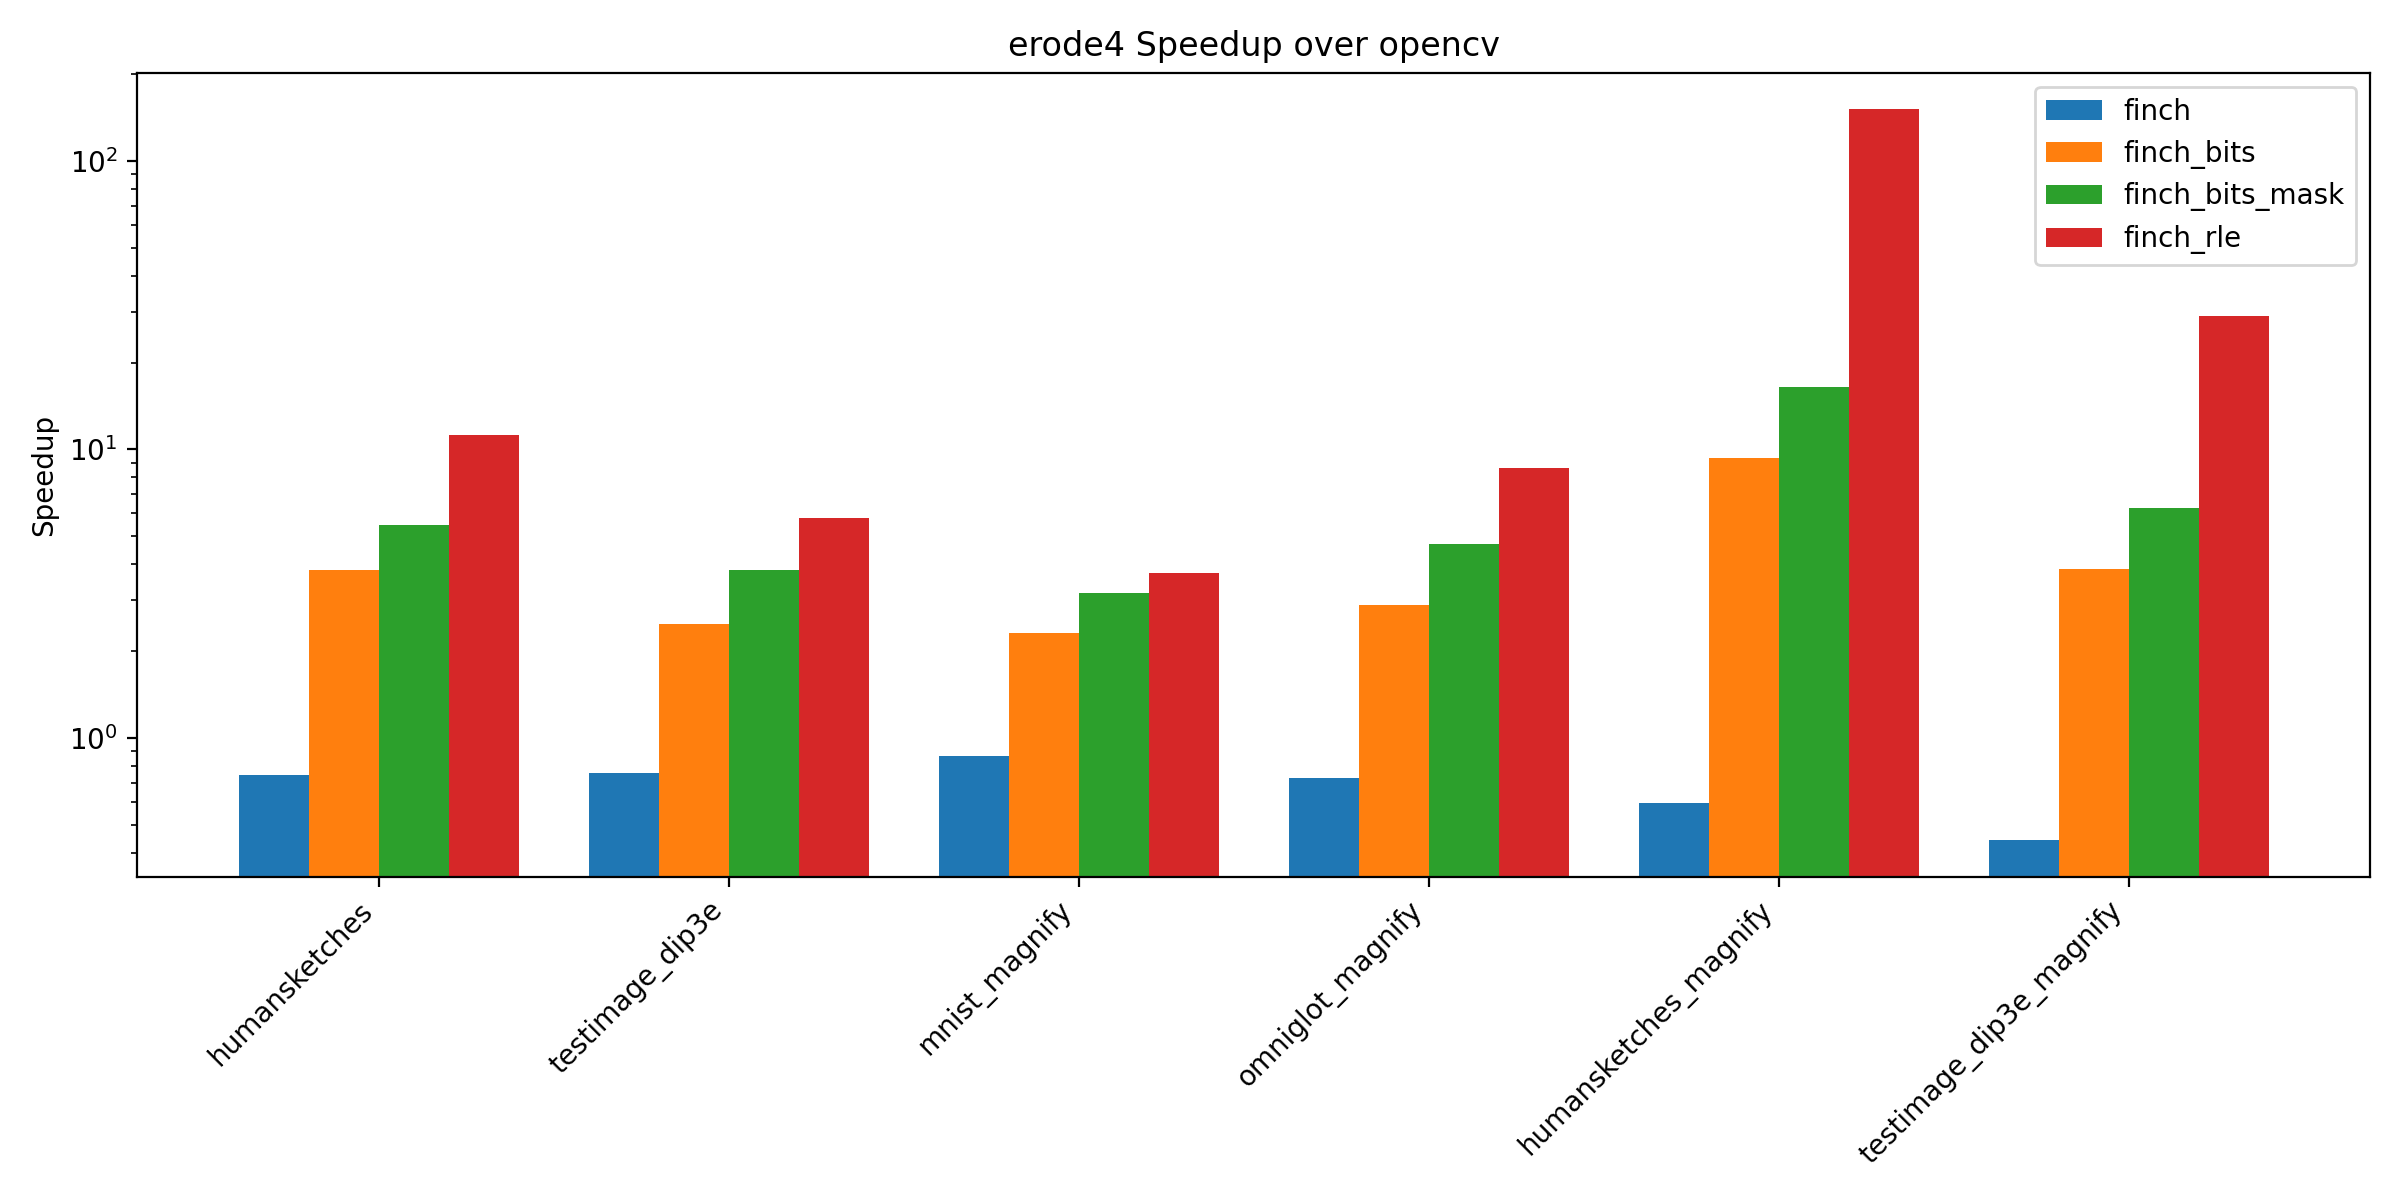
\includegraphics[width=\linewidth]{erode4_speedup_over_opencv.png}
    \caption{Performance of Finch on erosion task (4 iterations).}
\end{figure}

\begin{figure}
	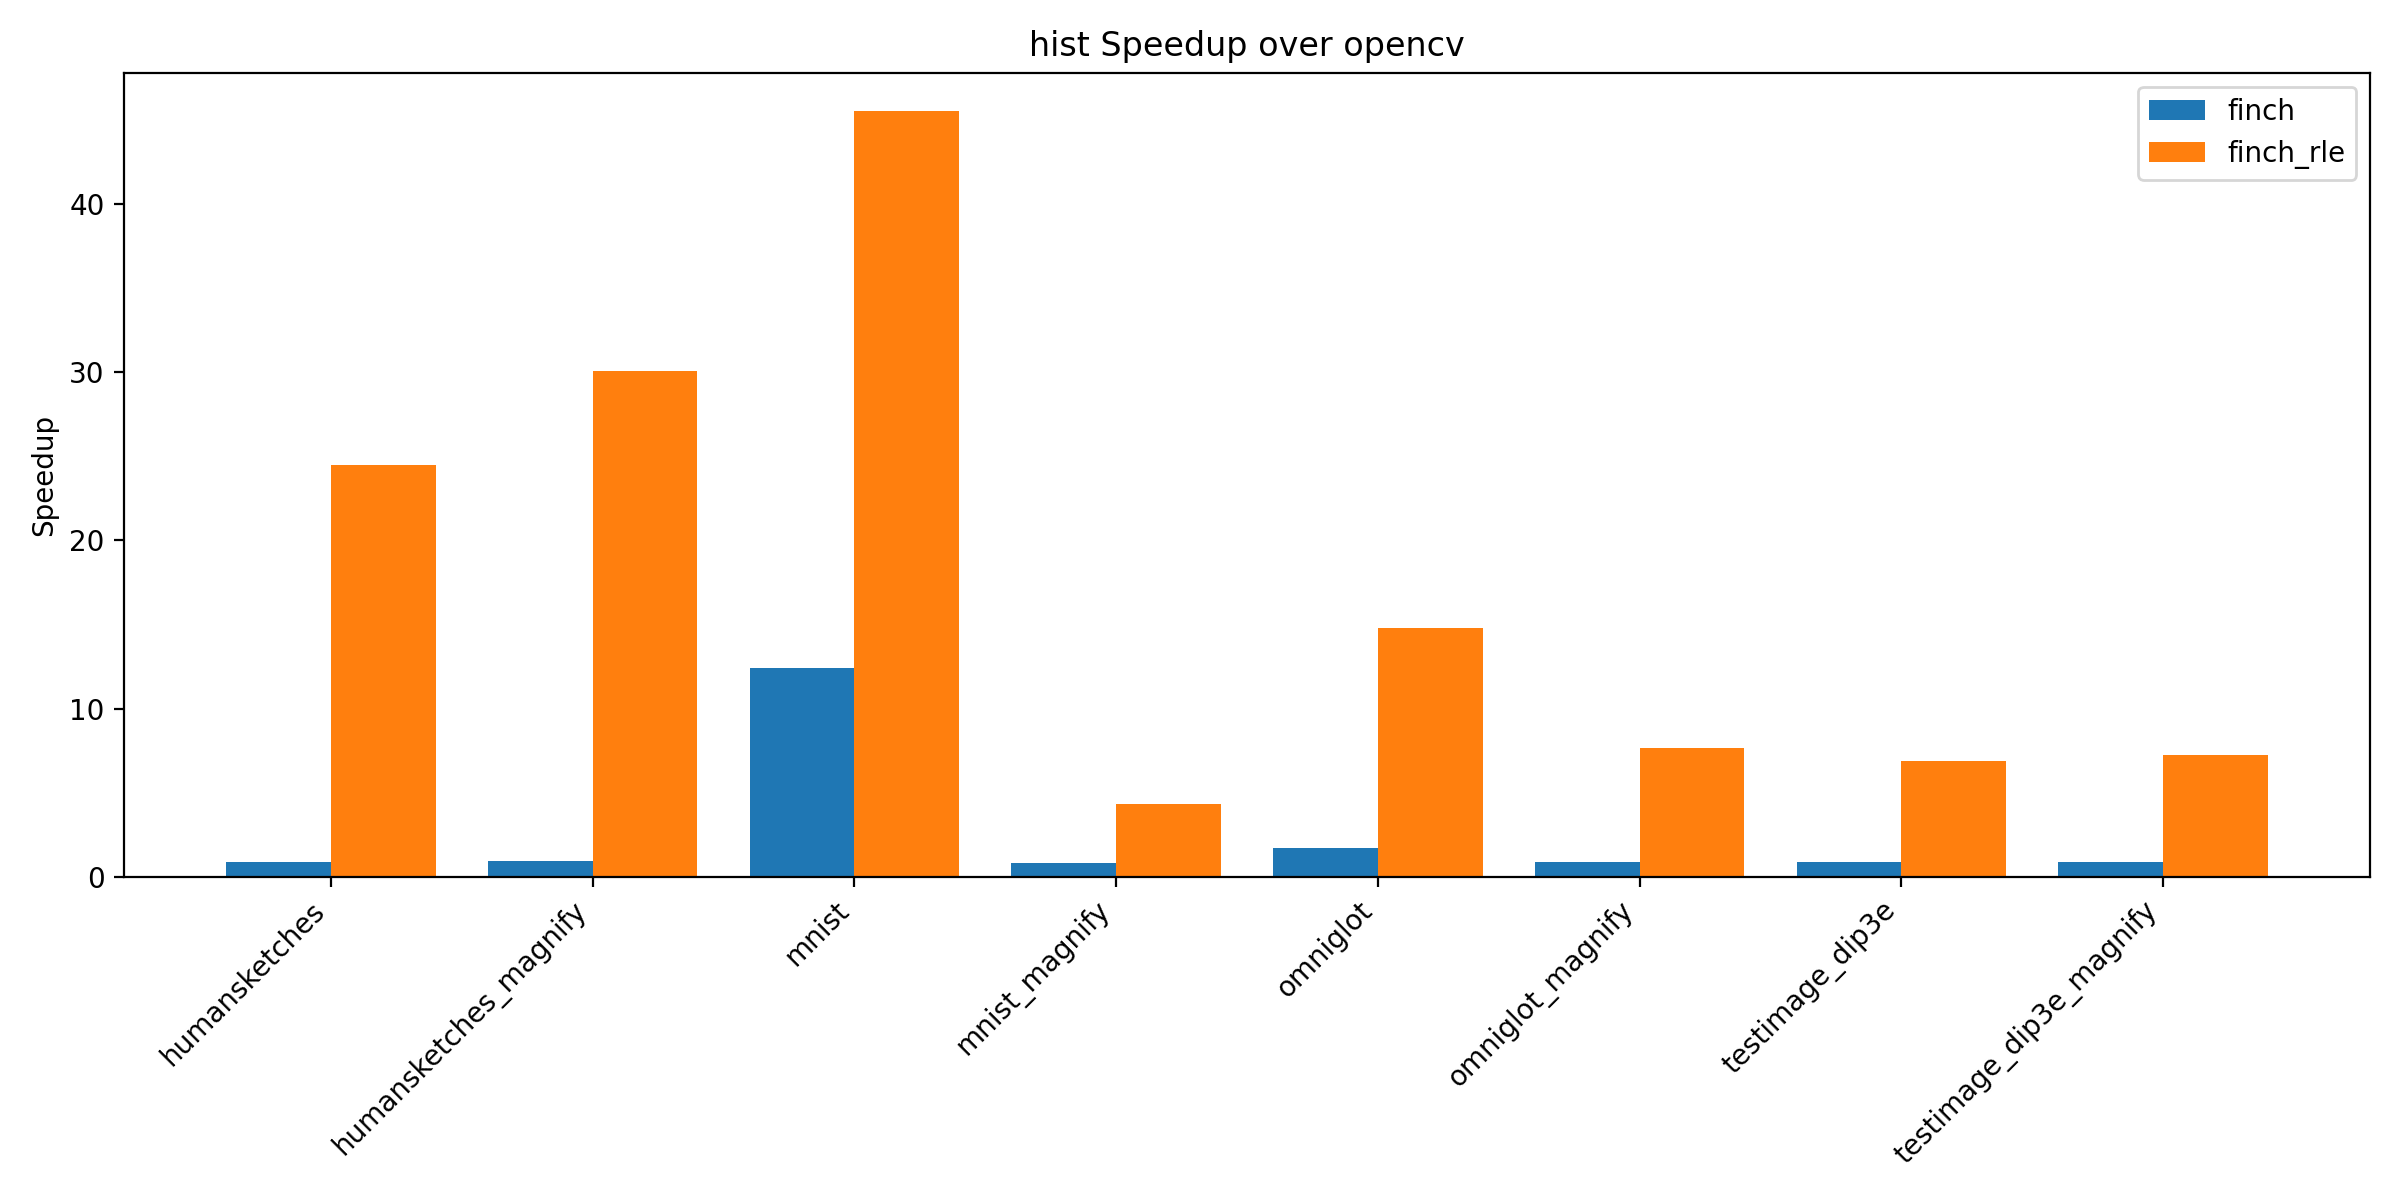
\includegraphics[width=\linewidth]{hist_speedup_over_opencv.png}
    \caption{Performance of Finch on masked histogram task.}
\end{figure}

\begin{figure}
	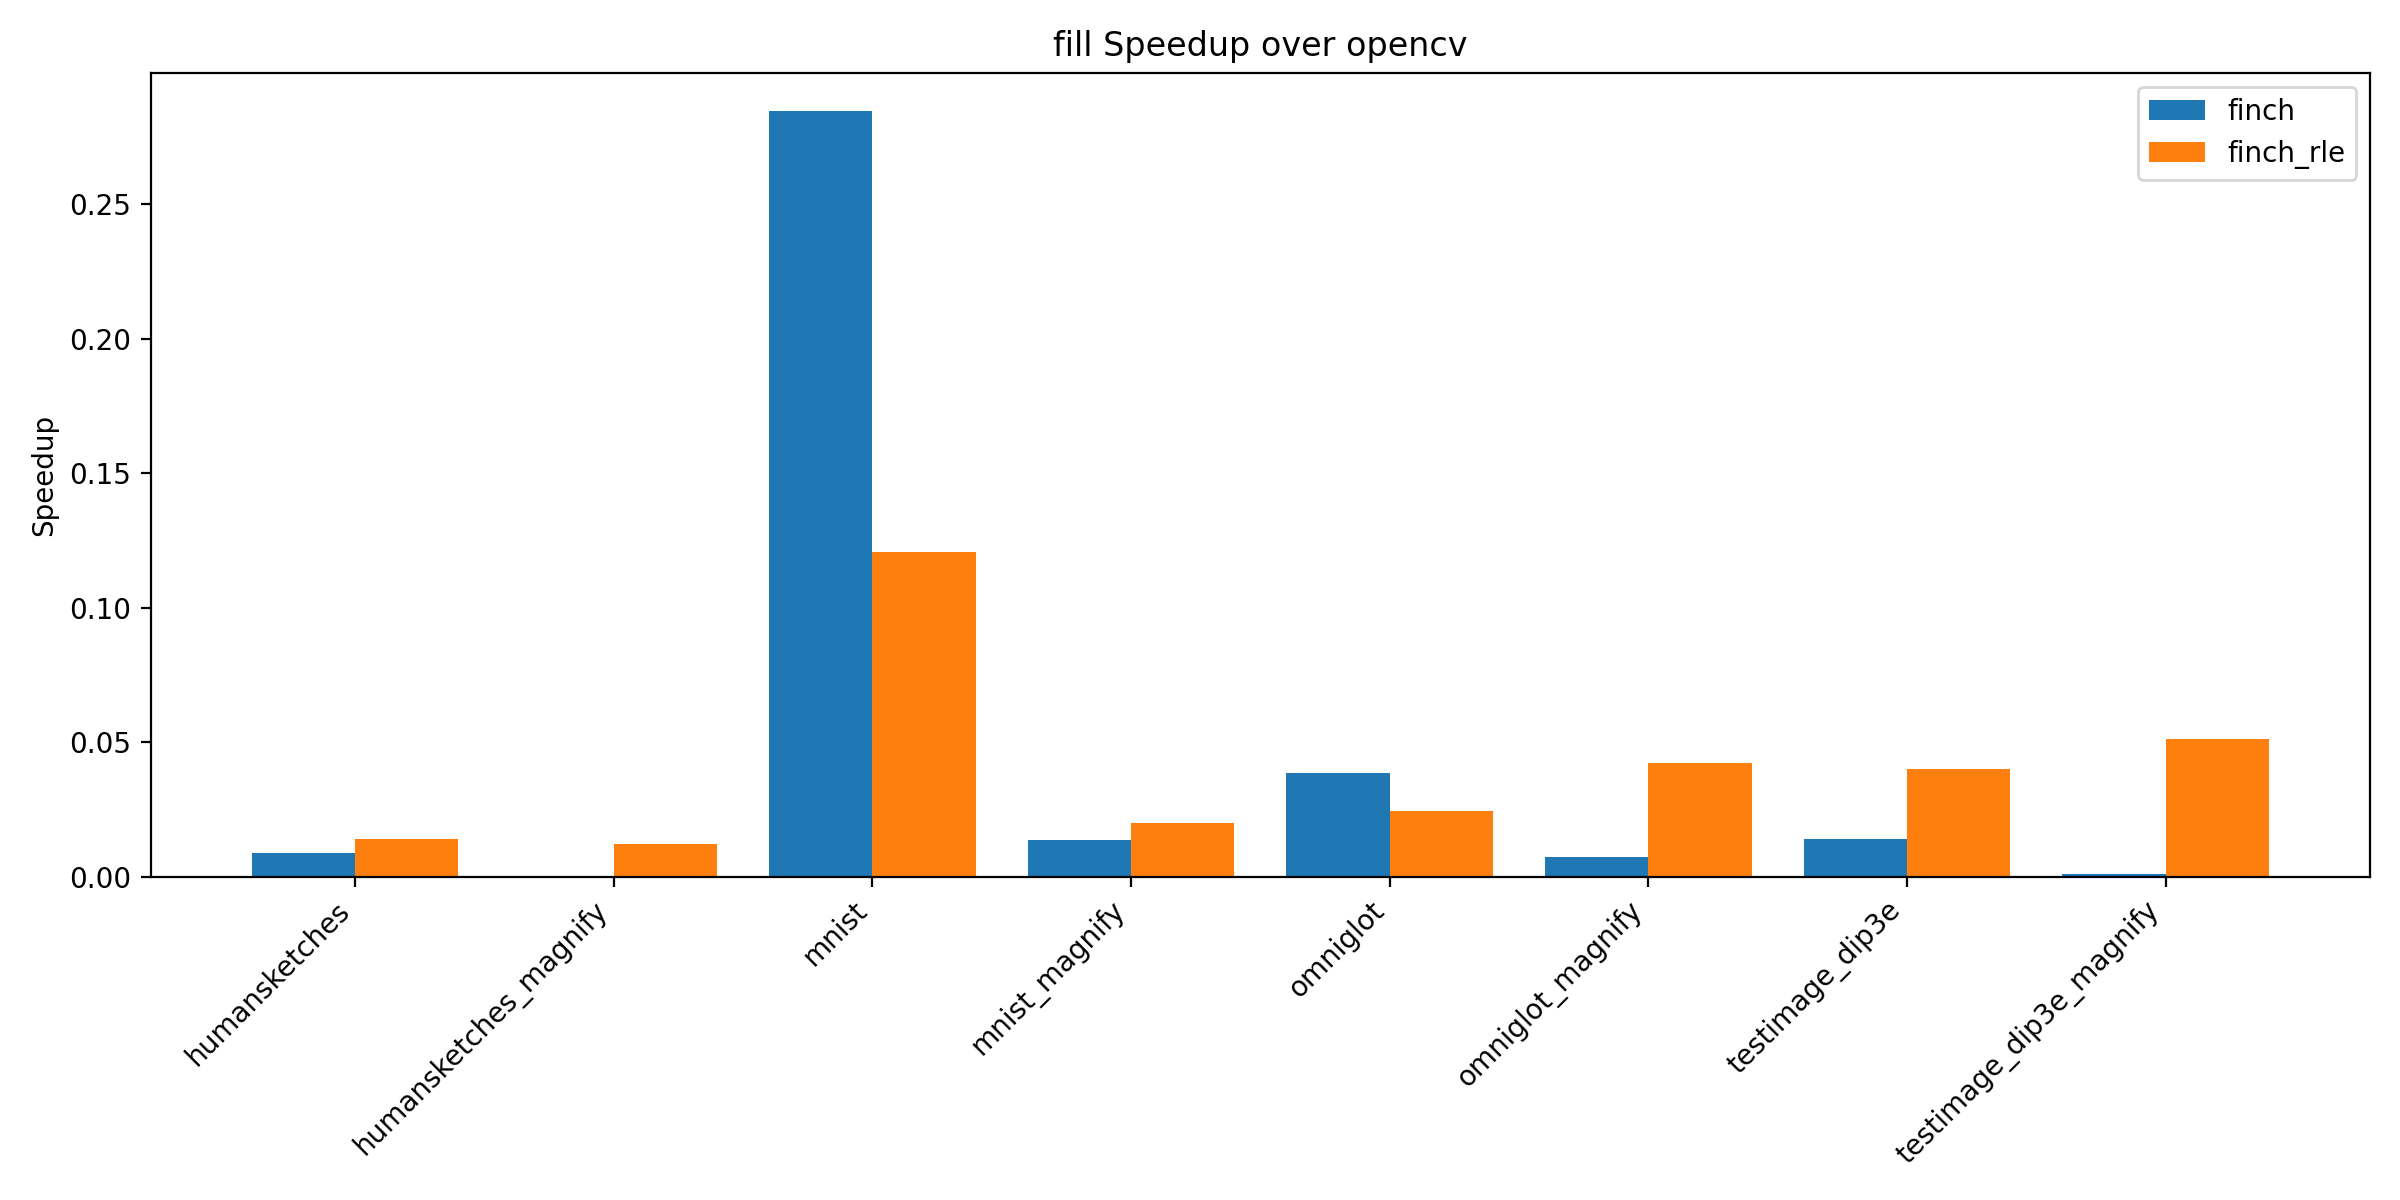
\includegraphics[width=\linewidth]{fill_speedup_over_opencv.png}
    \caption{Performance of Finch on flood fill task.}
\end{figure}

\subsubsection{Graph Analytics}
\begin{figure}
	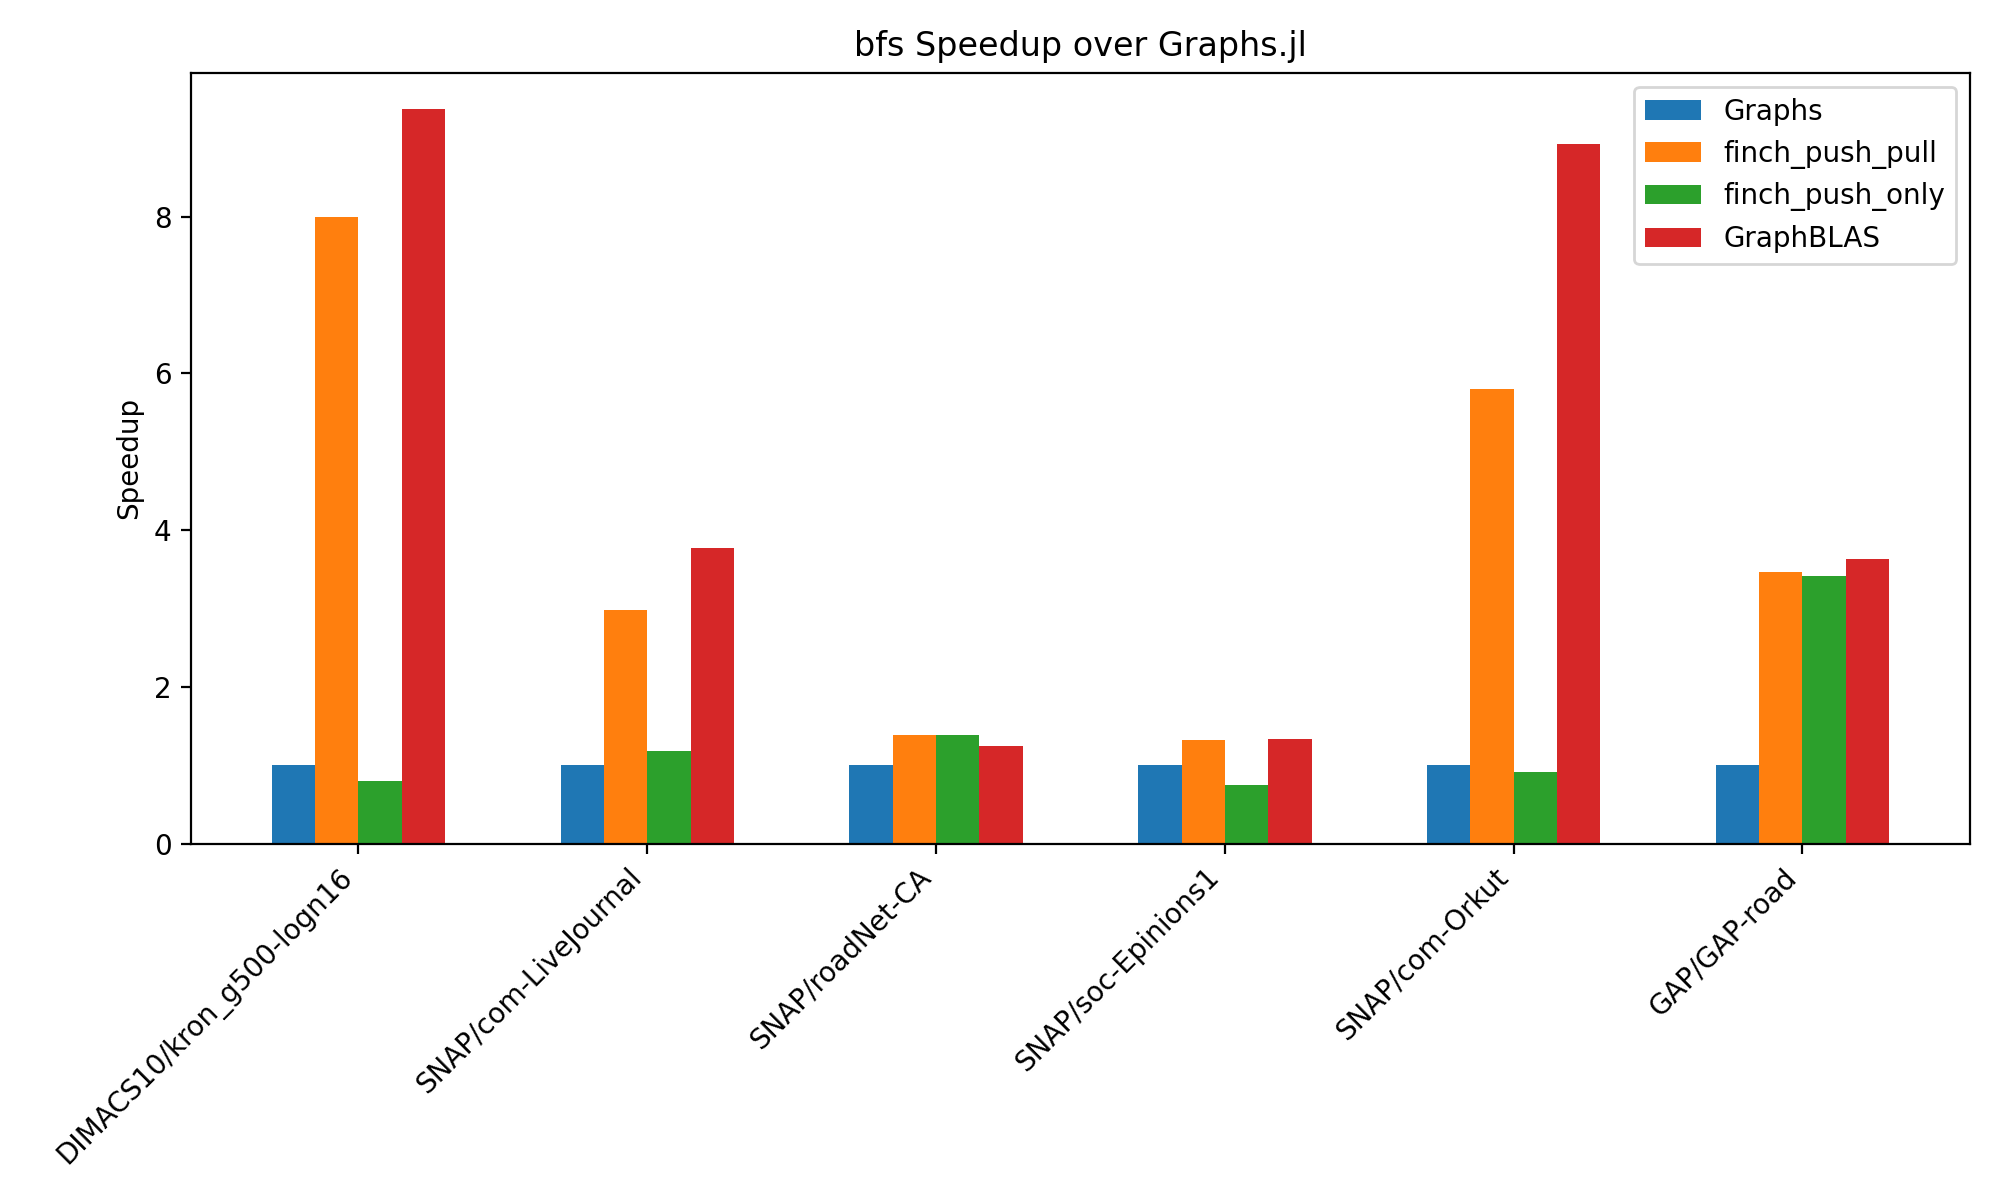
\includegraphics[width=\linewidth]{bfs_speedup_over_graphs.jl.png}
	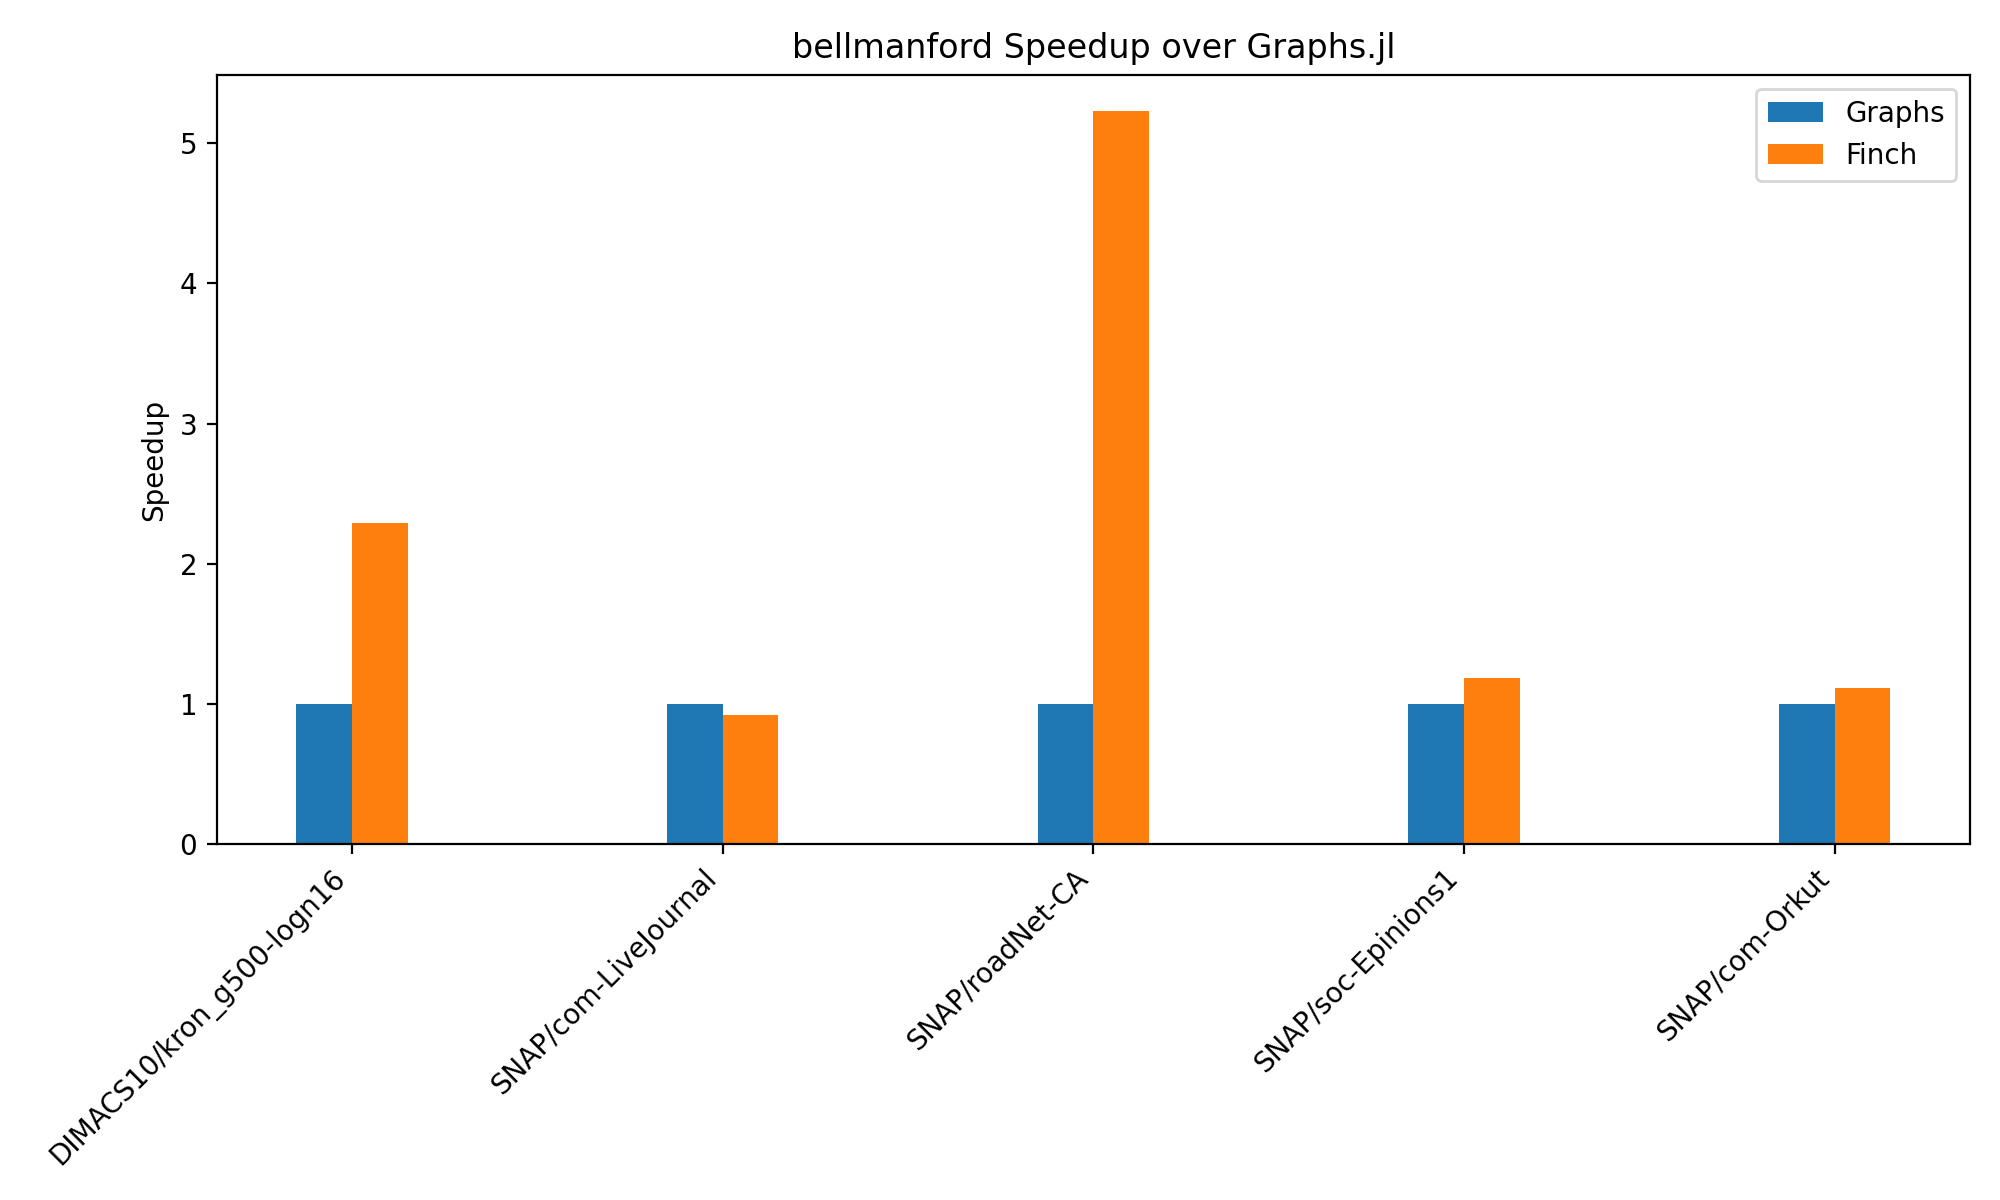
\includegraphics[width=\linewidth]{bellmanford_speedup_over_graphs.jl.png}
    \caption{Performance of graph apps across various tools.}
\end{figure}

\subsection{Implementing Numpy Array API in Finch}
\subsubsection{The Finch High-Level API (Needs a Name)}

\subsubsection{Finch Logic}

\subsubsection{Finch Interpreter}

\subsubsection{Lowering}
\subsubsection{Heuristic Optimization}

Find an example where fusing the python interface gives a big speedup over non-fused kernels.

matmul, mttkrp, repeated ttm, triangle counting, multiple pointwise,
in-place.
dot((v^t .* u), w)) vs. 
(v^t .* dot(u, w))

\bibliographystyle{alpha}
\bibliography{bibliography}

\end{document}